\chapter{Design}

In this section, the benchmark problem will be defined and mapped as DCOP, the framework design will be explained and the mapping of the algorithms on to the Signal/Collect framework will be described. Additionally, the design and considerations regarding the monitoring platform will be presented.

\section{Meeting Scheduling Problem}

\subsection{Formal Definition as DCOP}

The formulation of the meeting scheduling problem follows the basic definition of a distributed constraint optimization problem. Agents, variables and their relationships, as well as constraints shall be formulated. The components of a meeting scheduling problem are participants, their schedule, meetings and a given timeframe. For the sake of simplicity, it was decided to not take travel time between meetings or other parameters into consideration as certain researchers have done \cite{Grubshtein}. It was also decided to use utilities instead of costs. % FIXME find zitat

\theoremstyle{hardconstraint2}
\newtheorem{hardconstraint2}{Definition}
\begin{hardconstraint2}
Participant - has preferences and meeting he/she need to attend
\end{hardconstraint2}
\begin{hardconstraint2}
Meeting - has participants and needs to be held at an agreable time
\end{hardconstraint2}

%-------------------------- Variable  & Agent definition ------------------------------------------------
\begin{figure}[h!]
\includegraphics[width=300px]{graphics/variablemodell.png}
\caption{Different paradigms of mapping the meeting scheduling Problem \cite{Maheswarana}.}
\label{fig:variablemapping}
\end{figure}
Maheswarana et al. propose three different ways of mapping a meeting scheduling problem to variables (Figure \ref{fig:variablemapping}). TSAV (Time Slots As Variables), EAV (Event As Variables) and PEAV (Private Events As Variables). In EAV, every participant holds a private variable containing the timeslot that should be used for a meeting. PEAV is a modification of the EAV paradigm where agents don't share their local valuations \cite{Maheswarana,}. It was decided to follow the PEAV principle and model every meeting participation of an agent as one variable instead of using timeslots as variables. An agent therefore can hold multiple variables. This paradigm has also been tried by other researchers, which further established confidence in the decision \cite{Petcu2003}.
\begin{hardconstraint2}
Agent - holds one variable per meeting participation
\end{hardconstraint2}
\begin{hardconstraint2}
Variable - represents one meeting participation
\end{hardconstraint2}
%---------------------------- Domain & Value  definition -----------------------------------------------
A variable takes on a value \(s_{i} \in S_{i}\) in a defined problem domain \(D\). In the formulation of the meeting scheduling problem, the domain represents a finite set of timeslots and the variable assigns to one of these timeslots. This value represents the currently locally chosen timeslot for a specific meeting.
\begin{hardconstraint2}
Domain - holds a finite set of possible timeslots to schedule a meeting
\end{hardconstraint2}
\begin{hardconstraint2}
Value - assigns to a timeslot of the available timeslots in the Domain
\end{hardconstraint2}
%------------------------------ Constraints ---------------------------------------------------
From the problem definition in the background \& related work chapter one can derive soft and hard constraint. Soft constraints can possibly be constructed from the preferences of the participants and utilized to maximize the utility \cite{Franzin}. As the global utility should be optimized, the participants could as a consequence have a low local utility. Three differently weighted soft constraints have been defined to model preferences of agents. Preferred timeslots gain the highest utility, followed by free timeslots and blocked timeslots, which gain no value at all. Further, a timeliness soft constraint was defined that adds a higher utility to earlier timeslots. All of the soft constraints have unary relationships, i.e. are local. % FIXME \cite{Chapman2011} \cite{chun, andy 2003}\cite{mes, martijn 2007}\cite{BenHassine2007}\cite{Berger2008}
Additionally, two hard constraints with k-ary relationships to variable neighbours need to be formulated. The first would be an equality constraint for assigned values for a meeting timeslot between all variables related to a meeting. The second is a difference constraint of assigned values between all variables of an agent \cite{Farinelli, Angulo}.
\newline\newline
A local utility function \(u_{l}(s)\) would therefore include the sum of all soft constraints multiplied by the product of the hard constraints analogous to the global function defined in chapter {\ref{chap:background}}. These definitions and this form of a local utility function have been implemented at later stages of the thesis into the algorithms:
\[ u_{l}(s) = \prod_{\substack{hc_{k} \in HC}} u_{SC_{g}}(s) \bigg( \sum_{sc_{k} \in SC} u_{SC_{g}}(s) \bigg)\] 

\subsection{Problem Dataset Generation}

% ------------------------ Entscheidung, Verteidigung --------------------
During the course of the thesis, it was necessary to find a dataset for the benchmarking. The Frodo2\footnote{http://frodo2.sourceforge.net} framework or for example the the dataset from AAMAS, 2004 \footnote{http://teamcore.usc.edu/dcop/} do provide a couple of datasets for meeting scheduling. But because it was considered that in the benchmarks one would need to be able to produce problems with different densities and scale to high numbers of participants, as well as change constraints dynamically it was decided to generate meeting participations and agent schedules randomly. It was also chosen to limit the number of meeting participations per agent to keep the benchmarks more realistic analogously to \cite{Chun}.

\begin{itemize}
\item Schedules are blocked based on the percentage given trough the density parameter
\item Preferences for meetings are chosen randomly from free timeslots in the schedule
\item The number of meeting participations is chosen randomly from 1-5
\item The meeting participations are chosen at random
\end{itemize}

\section{Framework}

\subsection{Signal / Collect}

It was decided to build a specific framework for benchmarking dynamic problems. The foundation of the framework is the Signal/Collect framework \cite{Stutz2010}\footnote{http://uzh.github.io/signal-collect}, which is built on top of Akka\footnote{http://akka.io} and written in Scala\footnote{http://www.scala-lang.org}. It is a graph processing engine with a programming model that features vertices and edges. The vertices have a state and send signals along the edges to other vertices, which can contain any datatype. The signal usually is their state or in context of their state. The vertices collect the signals and perform a compution on the collected data, before adjusting their state according to the calculations and sending out the newly generated signal.  This model allows to reduce complex algorithms to a few lines of code and is applicable for many problems. The reason for choosing this framework in this thesis is the structural fit to distributed constraint optimization problems and the possiblity to add and remove vertices during runtime. This allows for dynamically changing problem computations. Further, the capability of running problems asynchronously or with synchronous signal steps and the possibility to distribute the system on multiple machines add to the advantages.

\subsection{Structure \& Functionality}
The considerations for the structure of the framework were that I needs to be hierarchical to allow different constraint optimization problems to be run. This mainly concerns the Vertices. For a basic convergence function and control parameters on the number of sent signals a \texttt{BasicVertex} has been implement. Further a \texttt{MeetingSchedulingVertex} has been implemented. This Vertex acts a generalization

It was decided to have a variable represent each meeting participation of a user and connect every of those variables of one agent to the agent vector, where meeting times are registered. This agent vector acts as an difference hard constraint between the participations of a user and is not a Signal / Collect edge, but a shared reference. Further, all variables attending a meeting also share a reference to the meeting vector where every agent shares his current preference which is in essence a equality hard constraint. 
The local utility function is based on the definitions in chapter 2.2. The reason why the utility function has been generalized on this level is because the structure has repeated itself in all three implemented algorithm approaches. It is further helpful for comparison to have the exact same utility function implemented.

 that includes a convergence function for meeting scheduling, the local utility function and data storage functions. 
To generalize dynamic change functions, a \texttt{DynamicVertex} was created, which implements methods for changing constraints and the value domain of the vertex. The concrete vertex implementations from the three approaches extends the \texttt{DynamicVertex}.

\subsection{Dynamics Controller}

The initial design consideration to introduce change to the constraints in the agents was to create a special vertex as part of the graph in Signal/Collect because the framework supports multiple types of vertices and messages in one graph execution. However, the vertex needed to be paused in the case of interval changes for a certain time and this caused errors during execution. Akka distributes multiple actors to the same thread and through pausing the dynamics vertex, other vertices were blocked. Through the abstractions in the Signal/Collect framework, it was not possible to gain access to the Akka dispatcher to schedule the activation of the vertex as a possible solution. It therefore was decided to run the changes controller in it's own thread alongside the graph execution.\newline\newline
The controller is first of all able to change constraints at a given interval and percentage (of all constraints in the problem). It is also possible to run a change only once. In the case of the meeting scheduling problem implementation this is only related to soft constraints as hard constraints can be handled by adding or removing variables with the second function. The variable change function also can be run at a certain interval or at one timepoint.  One can add parameters to create a new neighbourhood or use existing relationships and add new variables or remove existing one's. Instead of given by percentage, this change is defined by number. As a third function, the controller does change the domain in the whole problem for all agents. In the use case of meeting scheduling, this increases or reduces the available timeslots.

\subsection{Parameters \& Modes}
This framework was designed with the benchmarks in mind.  It should be possible to pass the general run parameters like which algorithm to use, which Signal/Collect run mode (synchronous/asynchronous) to use, normal run mode or dynamic variations (changeConstraints, changeVariable, changeDomain) with specific parameters. For testing, two test modes were implemented: SingleTest and MultiTest. Single Test is for single runs obviously and MultiTest allows to specifiy how many runs each specification should be doing to create a median of those runs, how much the agents respectively the meetings should increase after a specification has been processed and where to stop. By this, it is possible to explore an area of specifications. Finally, it should be possible to define different problems. For this thesis, the parameters for problem density (blocked timeslots percentage), timeslots, meetings and agents were defined.

\section{Mapping of DPOP}

The following sections describes the mapping of the graph structure of the DPOP algorithm and the behaviour of it's nodes to the Signal/Collect Framework  in regards to the meeting scheduling problem. The implementation is based on \cite{Petcu2003}.

\begin{figure}[h]
\includegraphics[width=200px]{graphics/dpop_graph}
\centering
\caption{An example DPOP pseudograph}
\label{fig:dpop_graph}
\end{figure}

hard constraint connection not show in image
cycles
A pseudo-tree arrangement of a graph G is a rooted tree with the same vertices as G and the property that adjacent vertices from the original graph fall in the same branch of the tree (e.g. X0 and X11 in Figure 1). Petcu2003


The process of the algorithm in short

\begin{algorithm}[H]
\caption{DPOP Util Message Handler}\label{euclid}
\begin{algorithmic}[1]
\State DPOP (X, D, R) \newline Each agent Xi executes:
\State $\textit{stringlen} \gets \text{length of }\textit{string}$
\State $i \gets \textit{patlen}$
\BState \emph{top}:
\If {$i > \textit{stringlen}$} \Return false
\EndIf
\State $j \gets \textit{patlen}$
\BState \emph{loop}:
\If {$\textit{string}(i) = \textit{path}(j)$}
\State $j \gets j-1$.
\State $i \gets i-1$.
\State \textbf{goto} \emph{loop}.
\State \textbf{close};
\EndIf
\State $i \gets i+\max(\textit{delta}_1(\textit{string}(i)),\textit{delta}_2(j))$.
\State \textbf{goto} \emph{top}.
\end{algorithmic}
\end{algorithm}

\begin{algorithm}[H]
\caption{DPOP Value Message Handler}\label{euclid}
\begin{algorithmic}[1]
\State DPOP (X, D, R) \newline Each agent Xi executes:
\State $\textit{stringlen} \gets \text{length of }\textit{string}$
\State $i \gets \textit{patlen}$
\BState \emph{top}:
\If {$i > \textit{stringlen}$} \Return false
\EndIf
\State $j \gets \textit{patlen}$
\BState \emph{loop}:
\If {$\textit{string}(i) = \textit{path}(j)$}
\State $j \gets j-1$.
\State $i \gets i-1$.
\State \textbf{goto} \emph{loop}.
\State \textbf{close};
\EndIf
\State $i \gets i+\max(\textit{delta}_1(\textit{string}(i)),\textit{delta}_2(j))$.
\State \textbf{goto} \emph{top}.
\end{algorithmic}
\end{algorithm}

Signal:
Collect:


\section{Mapping of MGM}

The following section describes the mapping of the graph structure of the Maximum-Gain Messaging algorithm and the behaviour of it's nodes described in chapter 2 to the Signal/Collect Framework in regards to the meeting scheduling problem. The implementation is based on \cite{Chapman2010}

\begin{figure}[h]
\includegraphics[width=250px]{graphics/mgm_graph}
\centering
\caption{An example MGM graph}
\label{fig:mgm_graph}
\end{figure}

Mapping the meeting scheduling problem to the structure of MGM was quite straightforward. The participant vertices of one meeting are all connected to each other through a Signal / Collect edge.

\begin{algorithm}[H]
\caption{MGM Pseudocode}\label{euclid}
\begin{algorithmic}[2]
\State currentReward = u(s = currentState, \(S_{v}\))
\For $\ k = 1:K $
\State $j stateGain(k) = u(s = k, sv) - currentREward$
\EndFor
\end{algorithmic}
\end{algorithm}

In the signal 

Collect:

 and send each other value messages.

\section{Mapping of MaxSum}

The following sections describe the mapping of the graph structure of  and the behaviour of it's nodes described in chapter 2 to the Signal/Collect Framework  in regards to the meeting scheduling problem. 

-- describe tests and thinking behind the chosen structure!!!! -> bipartite graph -> unary connections in factor graph should be possible
- had a problem with the property to send only to others with only 1 meeting.

\begin{figure}[h]
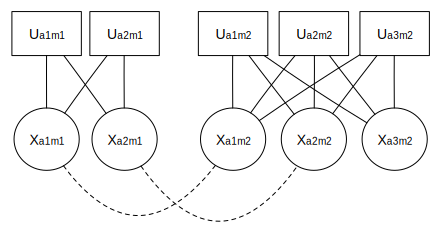
\includegraphics[width=250px]{graphics/maxsum_graph}
\centering
\caption{An example MaxSum graph}
\label{fig:maxsum_graph}
\end{figure}


This is the pseudocode of the MaxSum algorithm that has been used for the implementation \cite{Zivan2012}.

\begin{algorithm}[H]
\caption{Maxsum Pseudocode}\label{euclid}
\begin{algorithmic}[3]
\Procedure{MyProcedure}{}
\State $\textit{stringlen} \gets \text{length of }\textit{string}$
\State $i \gets \textit{patlen}$
\BState \emph{top}:
\If {$i > \textit{stringlen}$} \Return false
\EndIf
\State $j \gets \textit{patlen}$
\BState \emph{loop}:
\If {$\textit{string}(i) = \textit{path}(j)$}
\State $j \gets j-1$.
\State $i \gets i-1$.
\State \textbf{goto} \emph{loop}.
\State \textbf{close};
\EndIf
\State $i \gets i+\max(\textit{delta}_1(\textit{string}(i)),\textit{delta}_2(j))$.
\State \textbf{goto} \emph{top}.
\EndProcedure
\end{algorithmic}
\end{algorithm}

Signal:
Collect:

\section{Monitoring Platform}

The  storage and monitoring of the utilities, quality levels, conflicts and run statistics of the calculations is in bechmarks usually done by writing the results to a log file. It was decided to use an alternative method during the course of this thesis. Mainly because it was a desirable function  to automatically postprocess the results of the bechmarks on a detached machine and because real-time visibility was considered to be useful during the implementation of the algorithms.\newline Sending the results with non-blocking asynchronous HTTP requests\footnote{http://dispatch.databinder.net} to a restful API on a dedicated server was considered to be a viable option and worth trying out. The Play Framework\footnote{https://www.playframework.com} has been chosen for implementation because it is highly scalable and able to handle thousands of simultanous connections, is lightweight as well as non-blocking and allows to process results on-the-fly with code written in Java or Scala. It was also chosen because the Akka framework, which is also the foundation of Signal/Collect is tightly integrated and the actors concept is an integral part of the platform. For every benchmarking run, an actor is created that handles all the relevant incoming messages. It is therefore possible to run multiple benchmarks in parallel. The framework further allows to visualize the global utility of the graph in real-time via websockets. % FIXME bildli

%\includegraphics{graphics/monitoring}


